\section{HÀM SỐ MŨ, HÀM SỐ LÔGARIT}
\subsection{LÝ THUYẾT CẦN NHỚ}
\subsubsection{Hàm số mũ}
\begin{itemize}
	\item [\iconMT] \indam{Dạng:} $y=a^x$, trong đó $0<a \ne 1$.
	\begin{itemize}
		\item [\ding{172}] Tập xác định của hàm số $y=a^x$ là $\mathbb{R}$;
		\item [\ding{172}] Tập giá trị của hàm số $y=a^x$ là $(0;+\infty)$.
	\end{itemize}

	\item [\iconMT] \indam{Đồ thị hàm số $y=a^x$:}
	\begin{listEX}[1]
		\item [\ding{172}]\,\, Khi $a>1$ thì hàm số đồng biến trên $\mathbb{R}$.
		\item [\ding{173}]\,\, Khi $0<a<1$ thì hàm số nghịch biến trên $\mathbb{R}$.
		\item [\ding{174}]\,\, Đồ thị luôn qua $(0;1)$ và luôn nằm phía trên trục hoành.
		\end{listEX}
\hspace{1cm}
	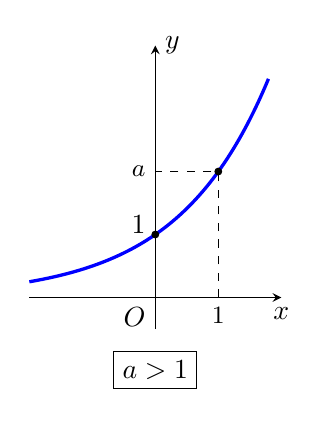
\begin{tikzpicture}[smooth,samples=300,scale=0.8,>=stealth]
	\draw[->] (-2,0)--(2,0) node[below]{$x$};
	\draw[->] (0,-0.5)--(0,4) node[right]{$y$};
	\draw (0,0) node[below left]{$O$};
	\draw[line width=1.2pt,color=blue,domain=-2:1.8] plot(\x,{2^(\x)});
	\draw[fill=black] (0,1) circle(1.5pt) (1,2) circle(1.5pt);
	\draw[dashed] (1,0)node[below]{\small$1$}--(1,2)--(0,2)node[left]{\small$a$};
	\node[below] at (0,-0.7) {\fbox{$a>1$}};
	\node[left] at (0,1.15) {$1$};
	\end{tikzpicture}
	\hspace{5cm}
	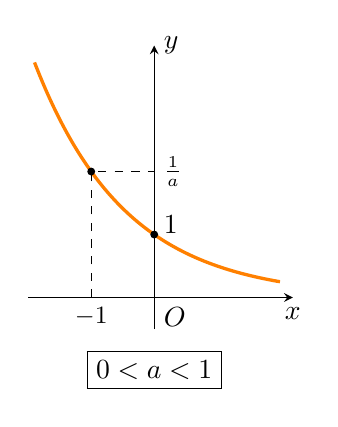
\begin{tikzpicture}[smooth,samples=300,scale=0.8,>=stealth]
	\draw[->] (-2,0)--(2.2,0) node[below]{$x$};
	\draw[->] (0,-0.5)--(0,4) node[right]{$y$};
	\draw (0,0) node[below right]{$O$};
	\draw[line width=1.2pt,color=orange,domain=-1.9:2] plot(\x,{0.5^(\x)});
	\draw[fill=black] (0,1) circle(1.5pt) (-1,2) circle(1.5pt);
	\draw[dashed] (-1,0)node[below]{\small$-1$}--(-1,2)--(0,2)node[right]{\small$\frac{1}{a}$};
	\node[below] at (0,-0.7) {\fbox{$0<a<1$}};
	\node[right] at (0,1.15) {$1$};
	\end{tikzpicture}
\end{itemize}
\subsubsection{Hàm số lôgarit}
\begin{itemize}
	\item [\iconMT] \indam{Dạng:} $y=\log_ax$, trong đó $0<a \ne 1$ và $x>0$.
	\begin{itemize}
		\item [\ding{172}] Tập xác định của hàm số $y=\log_ax$ là $(0;+\infty)$ ;
		\item [\ding{172}] Tập giá trị của hàm số $y=\log_ax$ là $\mathbb{R}$ .
	\end{itemize}
	\item [\iconMT] \indam{Đồ thị hàm số $y=\log_ax$:}
	\begin{listEX}[1]
		\item [\ding{172}]\,\, Khi $a>1$ thì hàm số đồng biến trên $(0; +\infty)$ 
		\item [\ding{173}]\,\, Khi $0<a<1$ thì hàm số nghịch biến trên $(0; +\infty)$ .
		\item [\ding{174}]\,\, Đồ thị luôn qua $(1;0)$ và luôn nằm bên phải trục tung.
	\end{listEX}
	\hspace{1cm}
	\begin{tikzpicture}[smooth,samples=300,scale=0.8,>=stealth]
	\draw[->] (-1,0)--(4,0) node[below]{$x$};
	\draw[->] (0,-2.5)--(0,2) node[right]{$y$};
	\draw (0,0) node[below left]{$O$};
	\draw[line width=0.8pt,color=violet,domain=0.2:3.2]plot(\x,{ln((\x))/ln(2)});
	\draw[fill=black] (1,0) circle(1.5pt) (2,1) circle(1.5pt);
	\draw[dashed] (2,0)node[below]{\small$a$}--(2,1)--(0,1)node[left]{\small$1$};
	\node[below] at (1,-2.6) {\fbox{$a>1$}};
	\node[below] at (1.1,0) {\small$1$};
	\end{tikzpicture}
	\hspace{5cm}
	\begin{tikzpicture}[smooth,samples=300,scale=0.8,>=stealth]
	\draw[->] (-1,0)--(4,0) node[below]{$x$};
	\draw[->] (0,-2)--(0,2.5) node[left]{$y$};
	\draw (0,0) node[below left]{$O$};
	\draw[line width=0.8pt,color=violet,domain=0.2:3.2]plot(\x,{ln((\x))/ln(0.5)});
	\draw[fill=black] (1,0) circle(1.5pt) (2,-1) circle(1.5pt);
	\draw[dashed] (2,0)node[above]{\small$\dfrac{1}{a}$}--(2,-1)--(0,-1)node[left]{\small$-1$};
	\node[below] at (1,-2.2) {\fbox{$0<a<1$}};
	\node[above] at (1.1,0) {\small$1$};
	\end{tikzpicture}
\end{itemize}